\documentclass[tikz,border=1pt]{standalone}
\usepackage{pgfplots}
\usepgfplotslibrary{fillbetween}
\begin{document}
	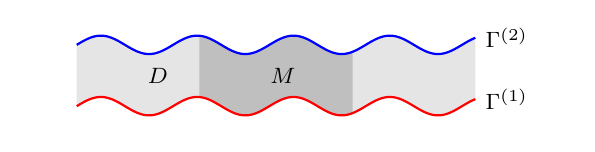
\begin{tikzpicture}
		\begin{axis}[xmax=8,axis lines=none,axis equal image=true]
			% two curves
			\addplot [blue,thick,smooth,samples=200,name path=gamma2,domain=0:6.5] {0.15*sin(4*\x r)+1} 
			node [black,right] {\footnotesize$\Gamma^{(2)}$};
			\addplot [red,thick,smooth,samples=200,name path=gamma1,domain=0:6.5] {0.15*sin(4*\x r)} 
			node [black,right] {\footnotesize$\Gamma^{(1)}$};
			
			% shading
			\addplot [gray!20] fill between [of=gamma2 and gamma1];
			\addplot [gray!50] fill between [of=gamma2 and gamma1,soft clip={domain=2:4.5}];
			
			% notations
			\draw (axis cs:1,0.5) node [right] {\footnotesize$D$};
			\draw (axis cs:3,0.5) node [right] {\footnotesize$M$};
		\end{axis}
	\end{tikzpicture}
\end{document}